\section{Thực nghiệm và kết quả}
\label{section4-experiment}

Phần này, trình bày một số kết quả dự kiến của đề tài khi hoàn thành.

\begin{itemize}
    \item Một hệ thống hadoop sẵn sàng để phục vụ storage, có quản lý truy cập dựa trên role-base access control. Công cụ quản lý thuận lợi, thực hiện bằng ứng dụng web như ví dụ tại các hình \ref{fig:sec5-ranger-portal}, \ref{fig:sec5-hadoop-portal}, \ref{fig:sec5-yarn-portal}
    \item Dữ liệu đánh giá hệ thống 
\end{itemize}

\begin{figure}
    \centering
    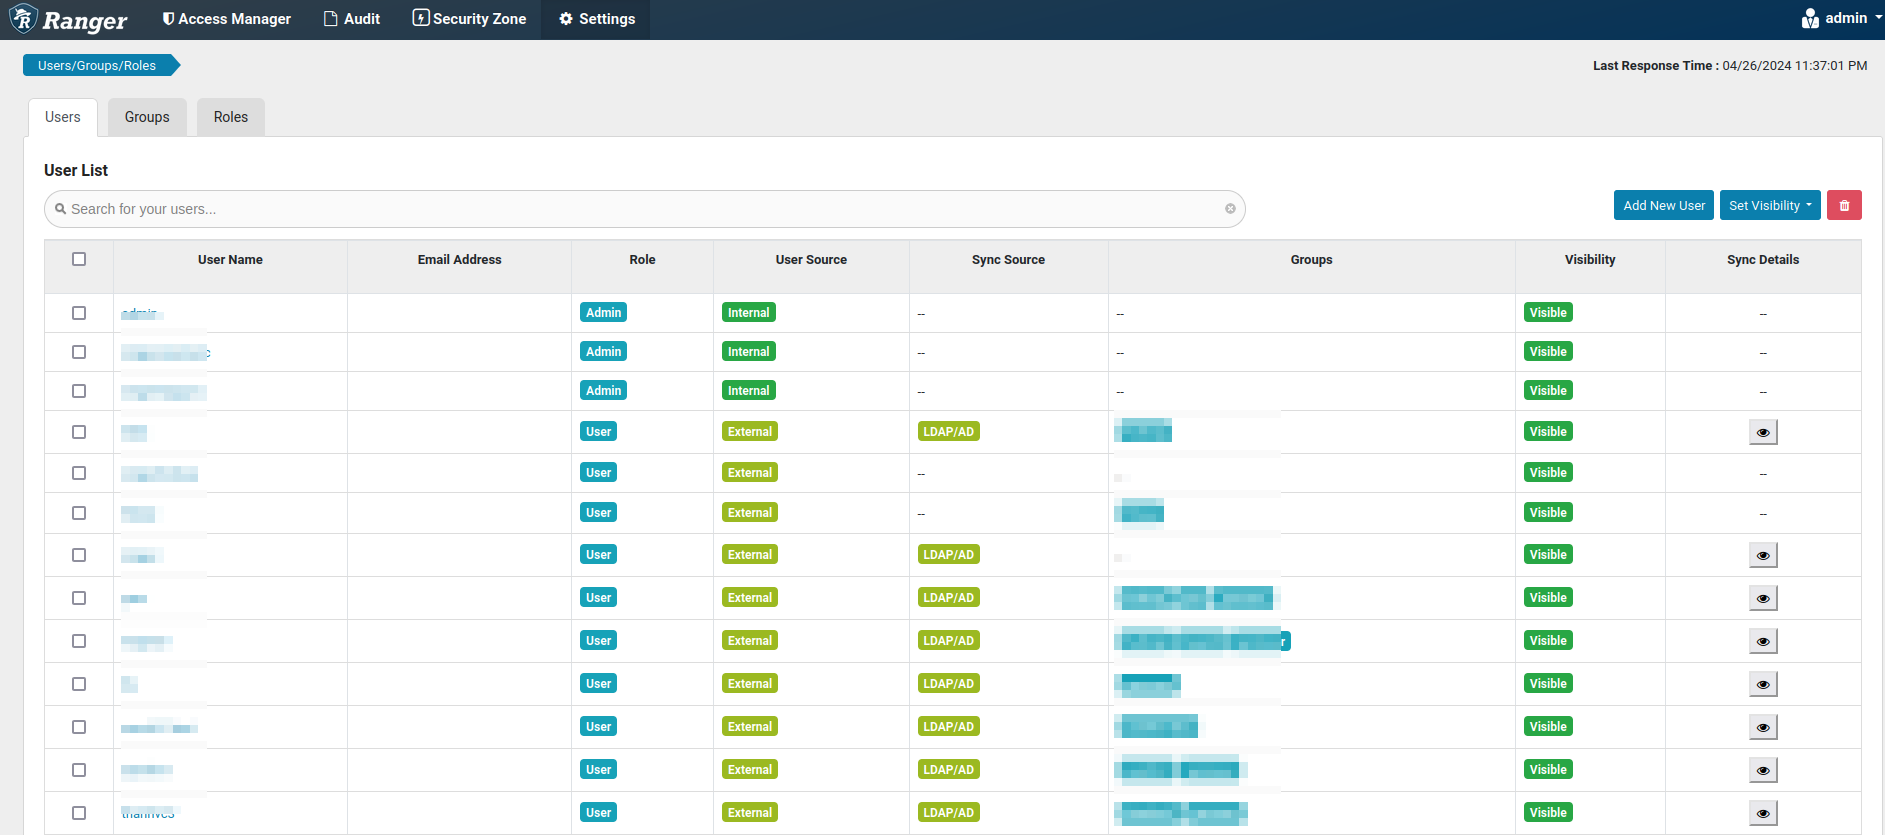
\includegraphics[scale=0.3]{section5/sec5-ranger-portal.png}
    \caption{Dự kiến giao diện quản lý người dùng trên Ranger}
    \label{fig:sec5-ranger-portal}
\end{figure}

\begin{figure}
    \centering
    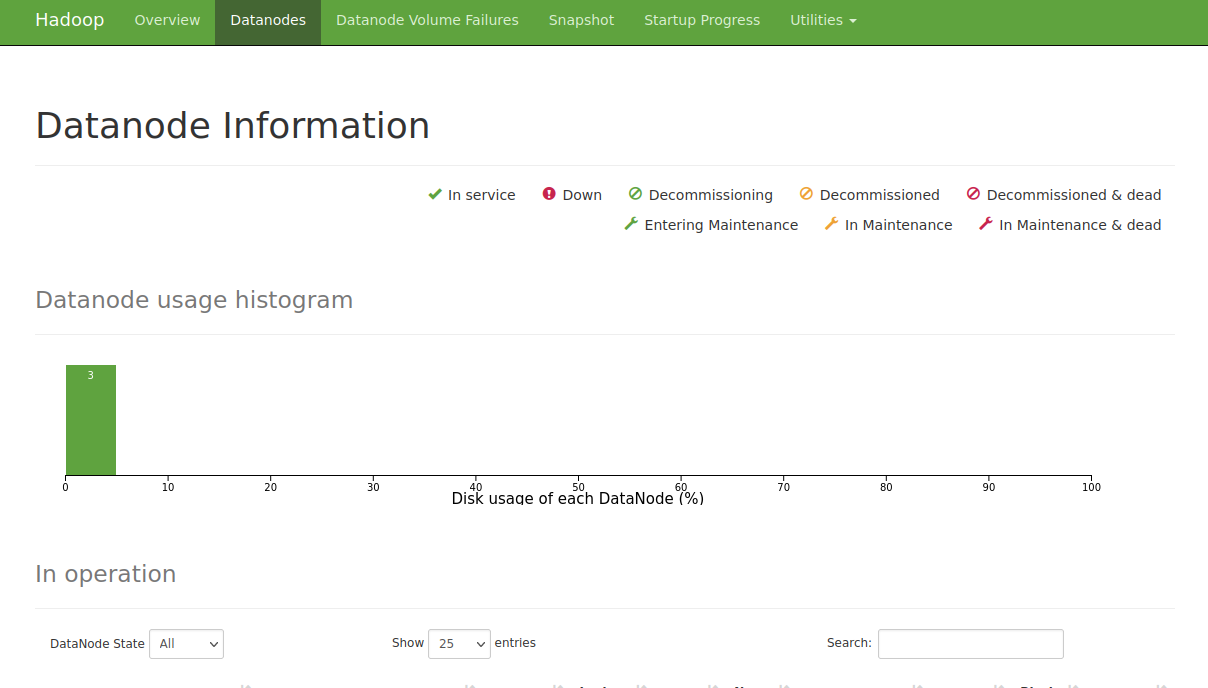
\includegraphics[scale=0.3]{section5/sec5-hadoop-portal.png}
    \caption{Dự kiến giao diện hadoop cluster}
    \label{fig:sec5-hadoop-portal}
\end{figure}

\begin{figure}
    \centering
    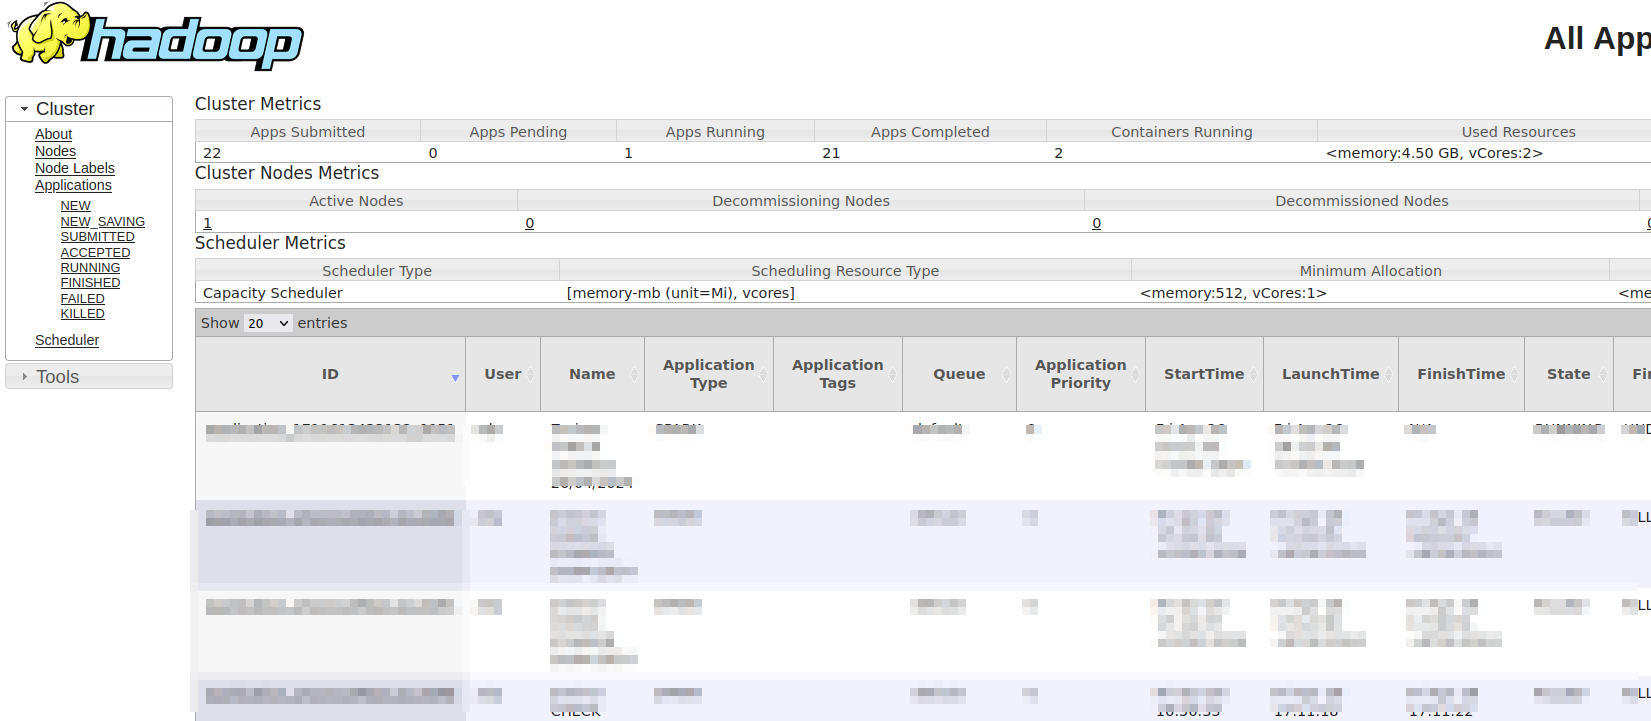
\includegraphics[scale=0.3]{section5/sec5-yarn-portal.png}
    \caption{Dự kiến giao diện yarn cluster}
    \label{fig:sec5-yarn-portal}
\end{figure}